\documentclass{article}
\usepackage[utf8]{inputenc}
\usepackage[T2A]{fontenc}
\usepackage{graphicx}
\graphicspath{ {images/} }
\title	{"Вкладені цики з лічильником y Scratch"}	\author{Толочко Ольга}
\date{14-11 2022}
\begin{document}
	\maketitle
	\newpage

\section*{Вкладені цикли з лічильником} 

\textbf {Цикл} - це фрагмент алгоритму, команди якого можуть виконуватися більше ніж один раз. 
Команди, які можуть виконуватися більше ніж один раз, утворюють \textbf {тіло циклу}.

	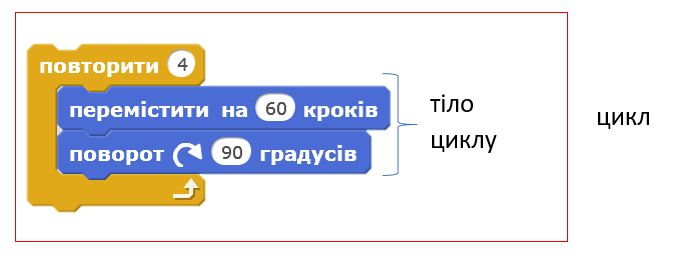
\includegraphics[width=0.75\textwidth]{1}
	
мал.1 Використання циклів
 \newline
Якщо серед команд тіла циклу є інші цикли, то такі фрагменти
алгоритму називають \textbf {вкладеними циклами}.
Цикл, який міститься в тілі іншого циклу, називають\textbf { внутрішнім}. 
А цикл, у тілі якого розміщено інший цикл, називають \textbf {зовнішнім}.

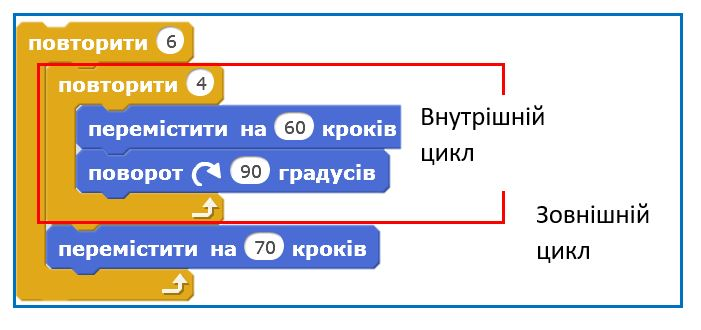
\includegraphics[width=0.75\textwidth]{2}

мал.2 Створення 6 квадратів, розміром 60 кроків на відстані один від одного на 70 кроків

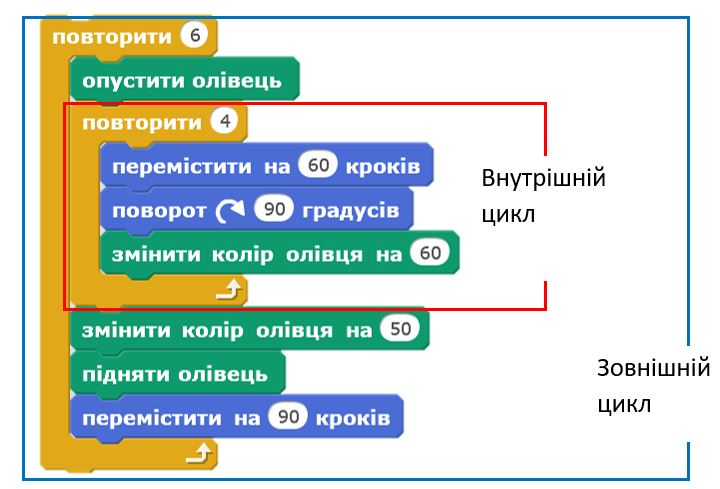
\includegraphics[width=0.65\textwidth]{3}

мал.3 Використання олівця для побудови 6 різнокольорових квадратів 
\newline

\textbf {Відео пояснення:} https://www.youtube.com/watch?v=wb5yf7wmFKo
\newline

\textbf {Завдання}
Скласти проект для малювання \textit{трьох кіл}, розміщених як це наведено на малюнку 4. 

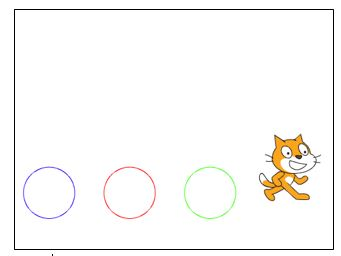
\includegraphics[width=0.65\textwidth]{4}

мал.4 Результат виконання проєкту
\newline

\textit{Для створення кола} використайте наведені блоки циклу

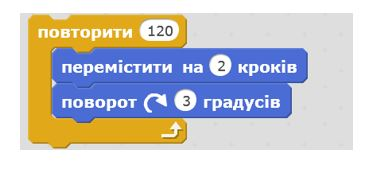
\includegraphics[width=0.65\textwidth]{5}

мал.5 Блоки для створення кола

\end{document}
